\documentclass[11pt]{article}
\usepackage[a4paper,margin=23mm]{geometry}
\usepackage{amsmath,amssymb,booktabs,graphicx,array,url,longtable}
\usepackage[section]{placeins}
\usepackage[hidelinks]{hyperref}
\setlength{\emergencystretch}{3em}
\title{How Much Does Corruption Training Help RGB-D Saliency Detection? A Three-Seed Study with an Audited Regional Router}
\author{[Author names and affiliations to be supplied]}
\date{}
\begin{document}
\maketitle

\begin{abstract}
Depth often improves salient object detection (SOD), yet missing or misregistered depth can increase mask error. We examine two responses: training an RGB-D candidate on a fixed mixture of synthetic depth degradations and selecting between that candidate and an independently trained RGB predictor with a regional utility router. A pooled 2,185-image NJU2K/NLPR training set was split into 1,749 fitting, 218 validation, and 218 calibration images. Three model seeds were evaluated on the official NJU2K (500) and NLPR (300) tests and on SIP (929), using clean depth, twelve graded degradations, and complete depth removal. Across the 13 degraded conditions, corruption training reduced candidate mean absolute error (MAE) relative to clean-depth-only training by $0.0052\pm0.0012$, $0.0052\pm0.0001$, and $0.0065\pm0.0045$ on NJU2K, NLPR, and SIP, respectively (mean $\pm$ standard deviation over seeds). Each of the nine seed--dataset paired image-bootstrap intervals for this comparison excluded zero. On clean depth, the RGB-D candidate also improved MAE over the RGB reference on all three datasets. The router recovered the RGB output under complete depth removal, but its selected-region fraction varied strongly among seeds and its mean positive harm exceeded a calibration budget of 0.005 under severe shifts on NJU2K and SIP. These results favor corruption-trained RGB-D prediction for the tested datasets and synthetic degradations at 320$\times$320 resolution. They do not establish a general safety guarantee or a consistent benefit from calibrated routing.
\end{abstract}
\noindent\textbf{Keywords:} RGB-D salient object detection; depth corruption; missing modality; utility routing; robustness evaluation.

\section{Introduction}
RGB-D salient object detection combines appearance and depth cues to segment prominent objects. Fusion, cooperative learning, attention, and depth calibration have improved how these cues are integrated \cite{pcf,dmra,jldcf,bbsnet,dcf}. Their success on clean depth does not mean that depth is always useful. A depth image can contain missing regions, blur, noise, or registration errors, so its value depends on both its quality and the RGB predictor's existing errors \cite{dqas,dqfm,dsn}.

We ask whether training a standard RGB-D detector with a fixed mixture of depth corruptions improves performance on degraded test depth. We then ask whether a regional router can use the observed RGB-versus-RGB-D error difference to select the better prediction. Candidate robustness and route calibration are separate questions: an accurate RGB-D predictor does not imply a reliable selector, particularly when the test corruption differs from the calibration distribution.

The system comprises an independently trained RGB reference, an RGB-D candidate, and a regional output router. We evaluate corruption training before assessing the router, so improvements in the candidate are not attributed to selection. The protocol uses three seeds and three test datasets, with deterministic perturbations, fixed-threshold and validity-only controls, paired image analyses, and measured inference costs.

\noindent\textbf{Contributions.} The contributions are specific to the implemented system and protocol. \emph{First}, it specifies a reproducible clean-only versus corruption-mixture training comparison, repeated for three seeds and evaluated on matched images under thirteen degraded conditions. \emph{Second}, it implements a candidate-relative regional utility target---the observed mask-error difference between two complete predictors---and an explicit RGB fallback when depth is absent. \emph{Third}, it audits threshold calibration using selection frequency, positive harm, fixed-threshold controls, and inference cost, exposing a severe-shift failure rather than asserting safety. The calibration budget does not imply a test-set guarantee. The work introduces neither a new backbone nor a physical, causal, or diffusion model, and it does not compare accuracy with external SOD systems under matched retraining.

\section{Related Work}
\subsection{RGB-D saliency and depth reliability}
RGB-D SOD has progressed from depth priors and cross-view transfer to progressive complementarity, multi-scale attention, and densely cooperative fusion \cite{globalprior,lbe,crossview,pcf,dmra,jldcf,bbsnet}. Other fusion designs include multi-path interaction, three-stream attention, hierarchical alternation, dynamic filtering, information conversion, collaborative learning, 3D convolution, and cross-modal refinement \cite{mmci,tanse,hainet,hdfnet,icnet,conet,rd3d,cirnet}. D3Net and survey work document the datasets and the variety of fusion designs \cite{d3net,survey2021}. These papers motivate the use of depth, but they do not substitute for a controlled comparison of the same candidate trained with and without depth degradation.

Fusion architecture determines whether an RGB-only alternative remains available at inference. Early feature fusion lets a network suppress depth internally, but the final RGB-D prediction has no explicit RGB-only alternative at inference. Cooperative and two-stream systems preserve modality-specific features longer, yet their reported output is still generally one jointly learned saliency map. An independently trained reference permits a measurable comparison on the same image: both alternatives produce complete maps before the selector acts. We use relatively small ResNet-18 predictors to keep the evaluation centered on depth training and selection rather than on a new encoder family.

Transformer and efficiency-oriented designs enlarge the architectural landscape \cite{vst,swinnet,caver,tritrans,singlestream,siamese,moadnet}. Depth-quality-aware SOD and depth-quality-inspired feature manipulation estimate whether the depth input should be trusted \cite{dqas,dqfm,dpanet,cdnet}. Depth calibration and selective fusion attempt to repair or downweight unhelpful depth \cite{dcf,calibrateddepth,twophase,dsn,cmms,ssf}. Distillation and efficient designs can reduce reliance on the depth pathway \cite{a2dele,mobilesal}. Our router instead uses the observed \emph{difference in mask error} between two complete predictors as its training target. The distinction lies in the supervised target, rather than in selective fusion as a general concept. Published results for these external methods are not included in our numeric tables because their checkpoints were not retrained and tested with our fixed corruptions.

Depth quality and the downstream value of a depth-dependent prediction are related but different quantities. A map with noisy edges may still rescue an RGB failure in an object interior; conversely, plausible depth may alter an already accurate RGB boundary. The candidate-relative target used here measures the change in mask error under a particular choice. A quality-aware model may perform better under the same protocol; none was retrained for this study. The present comparison isolates the target used to train our router, without ranking it against those models.

\subsection{Selective prediction and evaluation}
Selective prediction studies the trade-off between acting and abstaining \cite{selectivenet}; calibration studies distinguish a model score from its observed behavior \cite{guo2017}. Accordingly, we reserve a separate partition for threshold calibration. The threshold is optimized empirically and carries no finite-sample risk guarantee. We report MAE along with structure measure, weighted $F$-measure, and enhanced-alignment measure on clean resized masks \cite{smeasure,weighted,emeasure}. The primary corruption analysis uses MAE, because its per-image difference permits a direct paired comparison of training policies and routes.

The unit of uncertainty is an image, not a 16-pixel region or a severity realization. Regions inside one image share scene content, and the same image appears under multiple deterministic conditions. Resampling those dependent records as independent observations would make uncertainty intervals spuriously narrow. For the training-policy ablation, we first average each image over the thirteen degraded conditions, then resample image IDs within a fixed seed. Variation across three trained seeds is summarized separately rather than hidden inside the image bootstrap.

\section{Method}
\subsection{Reference and candidate predictors}
Let $I$ denote a normalized RGB image, $D\in[0,1]^{320\times320}$ its decoded depth image, $V$ a binary validity map, and $Y$ the binary saliency mask. The reference $R=f_R(I)$ and candidate $C=f_C(I,D,V)$ output probability maps. The reference uses one ImageNet-initialized ResNet-18 encoder \cite{resnet} and a four-level 32-channel top-down decoder. The candidate has separate RGB and two-channel $[D,V]$ ResNet-18 encoders. At each of four scales, projected RGB and depth features and resized validity are concatenated, passed through a 32-channel convolutional block, and decoded to a full-size mask. New blocks use convolution, GroupNorm, and ReLU. The depth encoder's first convolution is initialized from the channel mean of the pretrained RGB convolution, with the validity channel initialized to zero. Bilinear interpolation uses \texttt{align\_corners=False}.

The four encoder stages return feature maps at strides 4, 8, 16, and 32 with 64, 128, 256, and 512 channels. A one-by-one convolution maps each scale to 32 channels. In the RGB-D candidate, the two 32-channel projections and one resized validity channel form a 65-channel tensor, which a three-by-three block maps back to 32 channels. The decoder starts at the coarsest scale and repeatedly upsamples its feature, concatenates it with the next lateral feature, and applies another block. A one-by-one head and sigmoid produce a probability at the input resolution. The reference uses the analogous top-down decoder with only RGB features. The candidate's two encoders make it more expensive than the reference; neither uses a transformer or diffusion component. Figure~\ref{fig:architecture} summarizes the implemented predictor, utility-training, calibration, and inference paths; its example inputs and probability maps come from an identified NJU2K test image.

\begin{figure}[!tbp]
\centering
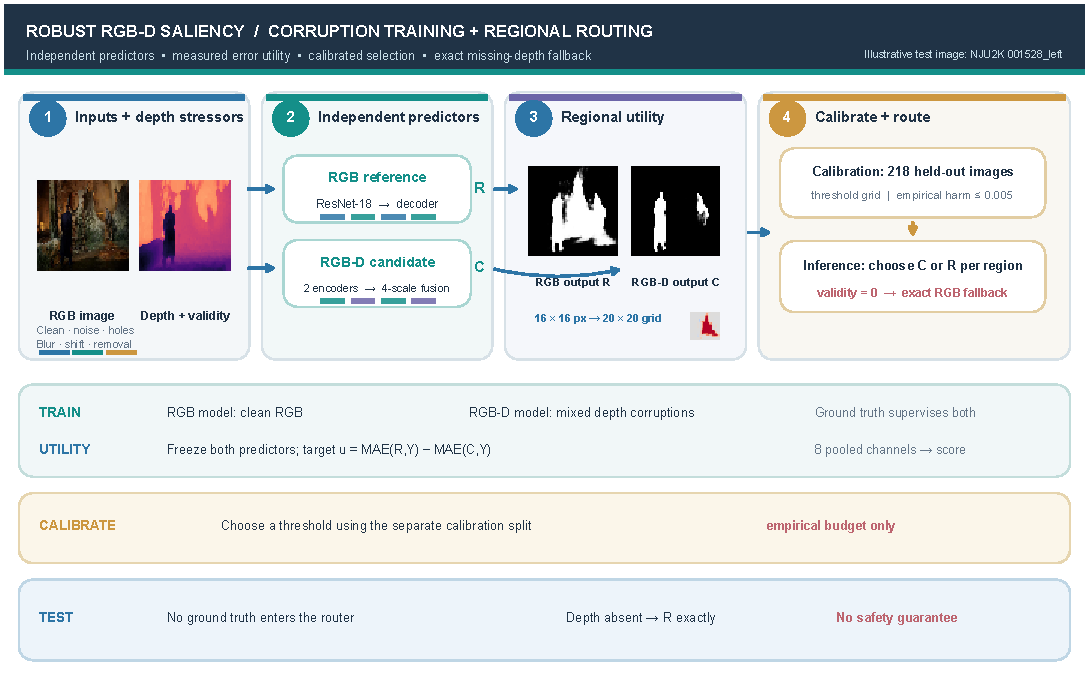
\includegraphics[width=\linewidth]{figure/fig1_architecture.pdf}
\caption{Implemented RGB-D saliency pipeline. The RGB reference and RGB-D candidate are independent predictors. Ground truth defines the regional error-difference target during router training only; inference uses frozen predictors and a threshold chosen on the separate calibration split. The thumbnails show NJU2K test image 001528\_left and its seed-17 predictions. The small utility-map illustration is computed from prediction errors against ground truth and is not an inference input.}
\label{fig:architecture}
\end{figure}

The reference is fitted on clean RGB; the candidate is fitted either on clean depth (ablation) or the specified corruption mixture (primary policy). Both use binary cross-entropy plus a soft-IoU term:
\begin{equation}
\mathcal L_{\rm seg}=\operatorname{BCE}(P,Y)+1-\frac{1}{N}\sum_{i=1}^{N}\frac{\sum_p P_{ip}Y_{ip}+1}{\sum_p(P_{ip}+Y_{ip}-P_{ip}Y_{ip})+1}.
\end{equation}
Their checkpoints are selected by clean validation MAE. The two training policies share the split, pretrained encoder source, optimizer, loss, and epoch budget, but the random decoder and fusion initializations were independently sampled; the comparison is therefore not an exact initialization-paired ablation.

Freezing the predictors keeps the router's utility target fixed during fitting. The reference and candidate are evaluated in inference mode while their predictions are cached for router training, and the routing head alone receives gradients. The clean-only training control starts a new candidate model instead of continuing the mixture-trained weights. The ablation therefore compares training policies on the same architecture and image pool, although independent random head initializations remain a potential confound. Repeating the comparison across three seeds describes, but does not eliminate, this variation.

\subsection{Regional utility router}
The predictors are frozen before router fitting. At each non-overlapping $16\times16$ region $b$, define reference and candidate errors $e_b^R=|b|^{-1}\sum_{p\in b}|R_p-Y_p|$ and $e_b^C=|b|^{-1}\sum_{p\in b}|C_p-Y_p|$. The target utility is $u_b=e_b^R-e_b^C$, transformed to $z_b=(u_b+1)/2$. Positive $u_b$ means that the candidate lowers the regional MAE.

The router receives eight pooled channels: $R$, $C$, $D$, $V$, $|R-C|$, the Bernoulli entropies of $R$ and $C$, and a validity-masked depth-gradient magnitude. Two 32-channel convolution--GroupNorm--ReLU blocks and a sigmoid output predict $q_b$. Mean squared error between $q_b$ and $z_b$ trains the router. At inference, ground truth is absent. For a threshold $t$, the candidate is selected when
\begin{equation}
a_b(t)=\mathbf 1\{2q_b-1>t\}\,\mathbf 1\{\overline V_b\geq0.5\},\qquad
P_p(t)=a_b(t)C_p+[1-a_b(t)]R_p\quad(p\in b).
\end{equation}
When depth is removed, $V=0$, hence $a_b=0$ and the implemented output equals $R$ on every pixel. This is a structural fallback property, not a statement that the RGB mask is always accurate.

The gate operates on a $20\times20$ grid, yielding 400 possible choices for a $320\times320$ mask. Selection is hard and spatially uniform inside each region. The selection frequency and each selected prediction can therefore be checked against the two complete outputs. It may also create seams at region boundaries and cannot adapt within a 16-pixel block. No smoothing or overlap correction was applied in the executed evaluation. Figure~\ref{fig:qualitative} displays examples of the resulting route masks and predictions.

\subsection{Empirical threshold selection}
For image $i$ and corruption condition $k$, let $\delta_{ik}(t)=\operatorname{MAE}(P_{ik}(t),Y_i)-\operatorname{MAE}(R_i,Y_i)$. The calibration script first averages $\delta_{ik}$ over the 14 fixed conditions for each image, then defines empirical benefit as minus the mean difference and empirical positive harm as the mean of $\max(0,\overline\delta_i)$. It chooses the threshold on the grid $\{-1,-0.98,\ldots,1\}$ with greatest empirical benefit subject to positive harm at most $\alpha=0.005$, breaking ties toward the larger threshold. Test harm is computed separately for each dataset and condition as $N^{-1}\sum_i\max(0,\delta_i)$. Because clipping occurs after condition averaging in calibration but separately by condition at test, these quantities have different scopes. Neither the optimization nor the budget guarantees a bound on an unseen corruption or individual image.

Regional and image-level harm should be distinguished. A selected region can be worse than the RGB reference even when the image-level routed result is better overall. The reported harm statistic clips the net image-level excess to zero and then averages it. It is not the sum of local selection errors. All router tables use this image-level definition. The corresponding selection fraction records how often the candidate was chosen; without it, a router that always returned RGB could appear harmless while providing no depth benefit.

\section{Experimental Protocol}
\subsection{Data and preprocessing}
The official NJU2K training split supplied 1,485 pairs and NLPR supplied 700 pairs. A fixed split seed of 2026 produced the pooled fitting, validation, and calibration partitions in Table~\ref{tab:data}; the same partitions were used for all model seeds. The official NJU2K and NLPR test splits and external SIP set were excluded from training and threshold selection. Local manifests record paths, IDs, datasets, and partitions. NJU2K source masks were checked against the local masks by exact pixel comparison.

The pooled split was made once and reused for all three model seeds; a seed changes model initialization, image order, flip pattern, training corruption assignment, and deterministic test corruption draws, but not official train/test membership. NJU2K and NLPR provide the fitting pool. SIP is used only for evaluation and thus probes transfer to another dataset without tuning its threshold. The numbers in Table~\ref{tab:data} are taken from saved JSONL manifests rather than inferred from a commonly cited split size. The validation set is used for choosing reference, candidate, and router checkpoints; the separate calibration set is reserved for choosing the route threshold.

\begin{table}[t]\centering\small
\caption{Actual image counts from the saved manifests. Validation selects model checkpoints; calibration selects only the router threshold.}
\label{tab:data}
\begin{tabular}{lrrrr}\toprule Dataset & Fit & Validation & Calibration & Official test\\\midrule
NJU2K & 1193 & 142 & 150 & 500\\
NLPR & 556 & 76 & 68 & 300\\
SIP & 0 & 0 & 0 & 929\\\midrule
Total & 1749 & 218 & 218 & 1729\\\bottomrule\end{tabular}
\end{table}

RGB is bilinearly resized to $320\times320$ and normalized with ImageNet channel statistics. Depth is decoded as an 8-bit grayscale image and divided by 255; there is no per-image min--max rescaling in the implementation. Ground truth is resized by nearest neighbor and binarized at 0.5. In the available benchmarks, $V$ initially contains ones. A seeded horizontal flip is applied during fitting. The implemented dataset loader derives that flip and the training corruption family deterministically from seed and image index, so an image's assigned corruption family remains fixed across epochs; this is an implementation-specific limitation rather than fresh online resampling.

\subsection{Depth perturbations and training}
The candidate training mixture comprises clean depth, Gaussian noise, a missing rectangle, Gaussian blur, integer displacement, and complete removal. Noise standard deviations are $0.02,0.05,0.10$ in normalized depth. Missing rectangles target fractions $0.10,0.25,0.40$; blur uses GaussianBlur radii $3,6,9$ pixels in the implementation; and shifts use magnitudes $2,5,10$ pixels in one of eight directions. Removal sets both depth and validity to zero. RGB and masks do not change under these depth-only sensitivity probes. Each family is assigned through the deterministic loader described above. Test perturbations are seeded by dataset, image ID, family, severity, replicate, and model seed, with one replicate per condition. The 14 test conditions are clean, three severities for each of four degradation families, and removal. No composed corruption or native sensor-failure test was run.

The implementation applies noise only to valid depth pixels and clips values to $[0,1]$. For holes, it samples a rectangular location and zeros both depth and validity there. Blur filters the product $D V$ and the validity mask separately before dividing, preventing invalid zeros from bleeding into nearby available depth; the input validity mask itself is retained. A shift moves depth and validity together by an integer offset while RGB and ground truth stay fixed. These deterministic operators act in normalized image coordinates. They model specific input failures, not a calibrated camera-noise process or a physically consistent change to the scene. Figure~\ref{fig:corruptions} illustrates the executed operators on a single identified NJU2K test sample while holding RGB fixed.

\begin{figure}[!tbp]
\centering
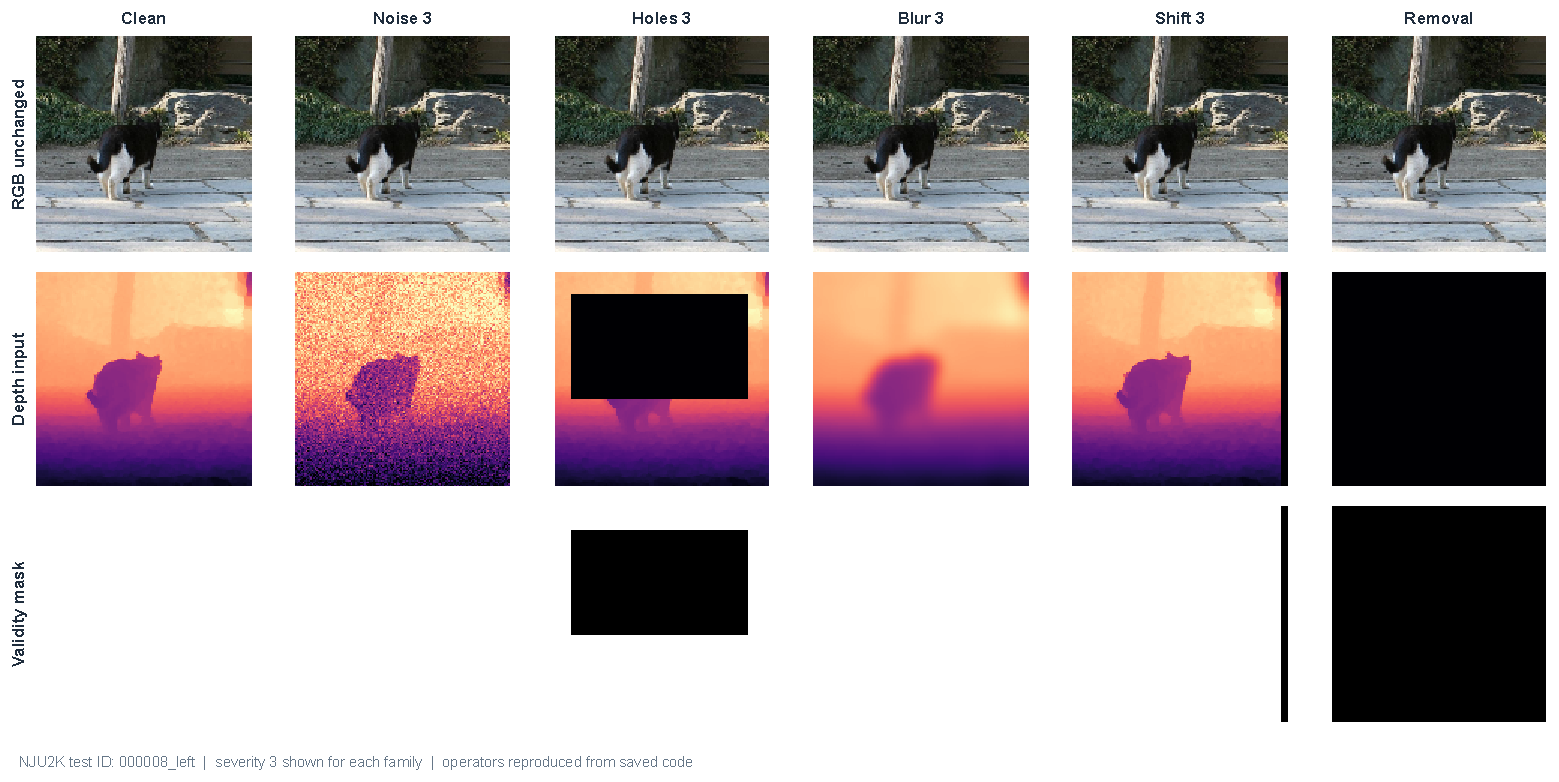
\includegraphics[width=\linewidth]{figure/fig2_depth_corruptions.pdf}
\caption{Synthetic depth perturbations used in the evaluation, illustrated on NJU2K test image 000008\_left. The rows show unchanged RGB, altered depth, and the corresponding validity mask. Severity 3 is shown for noise, holes, blur, and shift; removal zeroes depth and validity. The transformations act only on depth and validity, not on RGB or the saliency ground truth.}
\label{fig:corruptions}
\end{figure}

For each of seeds 17, 29, and 43, reference and candidate models were trained for 60 epochs each, followed by 60 epochs of router fitting in the executed training script. AdamW used learning rate $10^{-4}$, weight decay $10^{-4}$, and a cosine schedule for the segmentation stages. Batch size was 2. The recorded environment used PyTorch 2.14.0+cu130 and an NVIDIA GeForce RTX 3060 Laptop GPU. The clean-only candidate ablation repeated the candidate stage for 60 epochs and used the matching seed's test perturbations. The copied reference/router in its composite checkpoint was not retrained for that candidate; only \emph{candidate MAE} is interpreted in the training-policy ablation.

\subsection{Metrics and uncertainty}
All reported mask metrics are calculated at $320\times320$, not at native source resolution. Clean masks receive MAE, $S$-measure, weighted $F$-measure, and adaptive $E$-measure. Corruption results use MAE. Tables report the mean and sample standard deviation over three training seeds. For candidate-training contrasts, the same image and deterministic corruption are paired within each seed. Five thousand bootstrap resamples of image IDs yield the per-seed percentile 95\% intervals; the interval is conditional on the training seed and does not measure training-run uncertainty. The across-seed standard deviation is reported separately.

The candidate-training contrast defines a positive difference as
\begin{equation}
\Delta_{\rm train}=\mathrm{MAE}_{\rm clean-only}-\mathrm{MAE}_{\rm corruption-trained}.
\end{equation}
We calculate this difference on matched image/condition pairs, average across the thirteen degraded conditions for each image, and only then average across test images. The aggregation weights images equally within a dataset and conditions equally within an image. We report the complete-removal endpoint as part of those thirteen conditions and also separately because it exercises the structural RGB fallback. The clean condition is not mixed into the degraded average.

\section{Results}
\subsection{Clean-mask accuracy}
Table~\ref{tab:clean} shows that the corruption-trained RGB-D candidate improves mean clean MAE over the independently trained RGB reference on each test dataset. Routing changes these values little, and on SIP its MAE is slightly worse than the ungated candidate. Depth helps the candidate on clean images, whereas the benefit of routing is inconsistent.

The four clean metrics need not rank the models identically. For example, on NJU2K the routed MAE is lower than the candidate MAE by only 0.0002, while its mean structure measure is slightly lower. On NLPR the routed MAE and adaptive $E$ are slightly better than those of the candidate, but the differences are small relative to a typical change between trained seeds. On SIP the candidate is better than routing in MAE and weighted $F$. The mixed rankings offer no evidence that utility calibration systematically improves segmentation. The per-seed clean results are retained in the evaluation CSV files rather than reduced to a single favorable ranking.

\begin{table}[t]\centering\small
\caption{Clean test results at $320\times320$, means over three seeds. MAE is lower when better; $S$, weighted $F$ ($F^w$), and adaptive $E$ are higher when better. Per-seed values remain in the evaluation CSV files.}
\label{tab:clean}
\begin{tabular}{llrrrr}\toprule Dataset & Predictor & MAE & $S$ & $F^w$ & $E$\\\midrule
NJU2K & RGB reference & .0557 & .8710 & .8339 & .9012\\
 & RGB-D candidate & .0479 & .8872 & .8589 & .9054\\
 & Calibrated router & .0477 & .8867 & .8594 & .9072\\\midrule
NLPR & RGB reference & .0316 & .8971 & .8478 & .9387\\
 & RGB-D candidate & .0273 & .9091 & .8703 & .9490\\
 & Calibrated router & .0269 & .9088 & .8708 & .9500\\\midrule
SIP & RGB reference & .0699 & .8335 & .7826 & .8954\\
 & RGB-D candidate & .0567 & .8645 & .8289 & .9110\\
 & Calibrated router & .0570 & .8620 & .8273 & .9109\\\bottomrule\end{tabular}
\end{table}

\subsection{Corruption training as the primary robustness result}
Table~\ref{tab:ablation} directly contrasts the candidate trained on the depth-corruption mixture with the clean-only candidate. The mean across all 13 degraded conditions favors corruption training on NJU2K, NLPR, and SIP in each of the three seeds. The 95\% paired image-bootstrap interval for the mean difference excludes zero for all nine seed--dataset combinations. This result concerns the tested training policy and degradations. The intervals do not address the independently sampled decoder and fusion initializations. Under clean depth, the trade-off is dataset-dependent: the clean-only model tends to have lower MAE on NJU2K and SIP, while NLPR shows little change.

Corruption training helps on all three datasets, although the gain varies. NJU2K differences range from 0.0042 to 0.0065 across seeds, and NLPR differences cluster around 0.0052. SIP differences are 0.0039, 0.0040, and 0.0117, so the three-seed mean masks variation on the external test set. Table~\ref{tab:seedablation} lists each fit with a paired image interval. The intervals exclude zero within a fixed model seed; they are not a formal probability statement about an unbounded population of retrainings.

The clean-only candidate is a substantive control. It uses the same pretrained source, architecture, fitting set, 60-epoch budget, and clean validation selection rule. Its performance on clean NJU2K and SIP can be as good as, or better than, the mixture-trained candidate. The degraded-condition gain therefore comes with a possible clean-depth cost. The remaining initialization mismatch motivates a future run that saves one common initial candidate state and branches the two training policies from that exact state.

\begin{table}[t]\centering\small
\caption{Candidate MAE averaged equally over the 13 degraded conditions; mean $\pm$ sample SD over seeds 17, 29, and 43. $\Delta=$ clean-only minus corruption-trained MAE, so positive $\Delta$ favors corruption training.}
\label{tab:ablation}
\begin{tabular}{lrrr}\toprule Dataset & Corruption-trained & Clean-only & $\Delta$\\\midrule
NJU2K & $.0503\pm.0014$ & $.0555\pm.0018$ & $.0052\pm.0012$\\
NLPR & $.0289\pm.0009$ & $.0341\pm.0009$ & $.0052\pm.0001$\\
SIP & $.0614\pm.0033$ & $.0679\pm.0054$ & $.0065\pm.0045$\\\bottomrule\end{tabular}
\end{table}

Figure~\ref{fig:robustness} shows the severity-dependent candidate MAE for each corruption family and dataset. The individual-seed traces are visible behind the three-seed means and standard deviations, making the clean-only versus mixture-trained comparison auditable without treating test images as independent training runs.

\begin{figure}[!tbp]
\centering
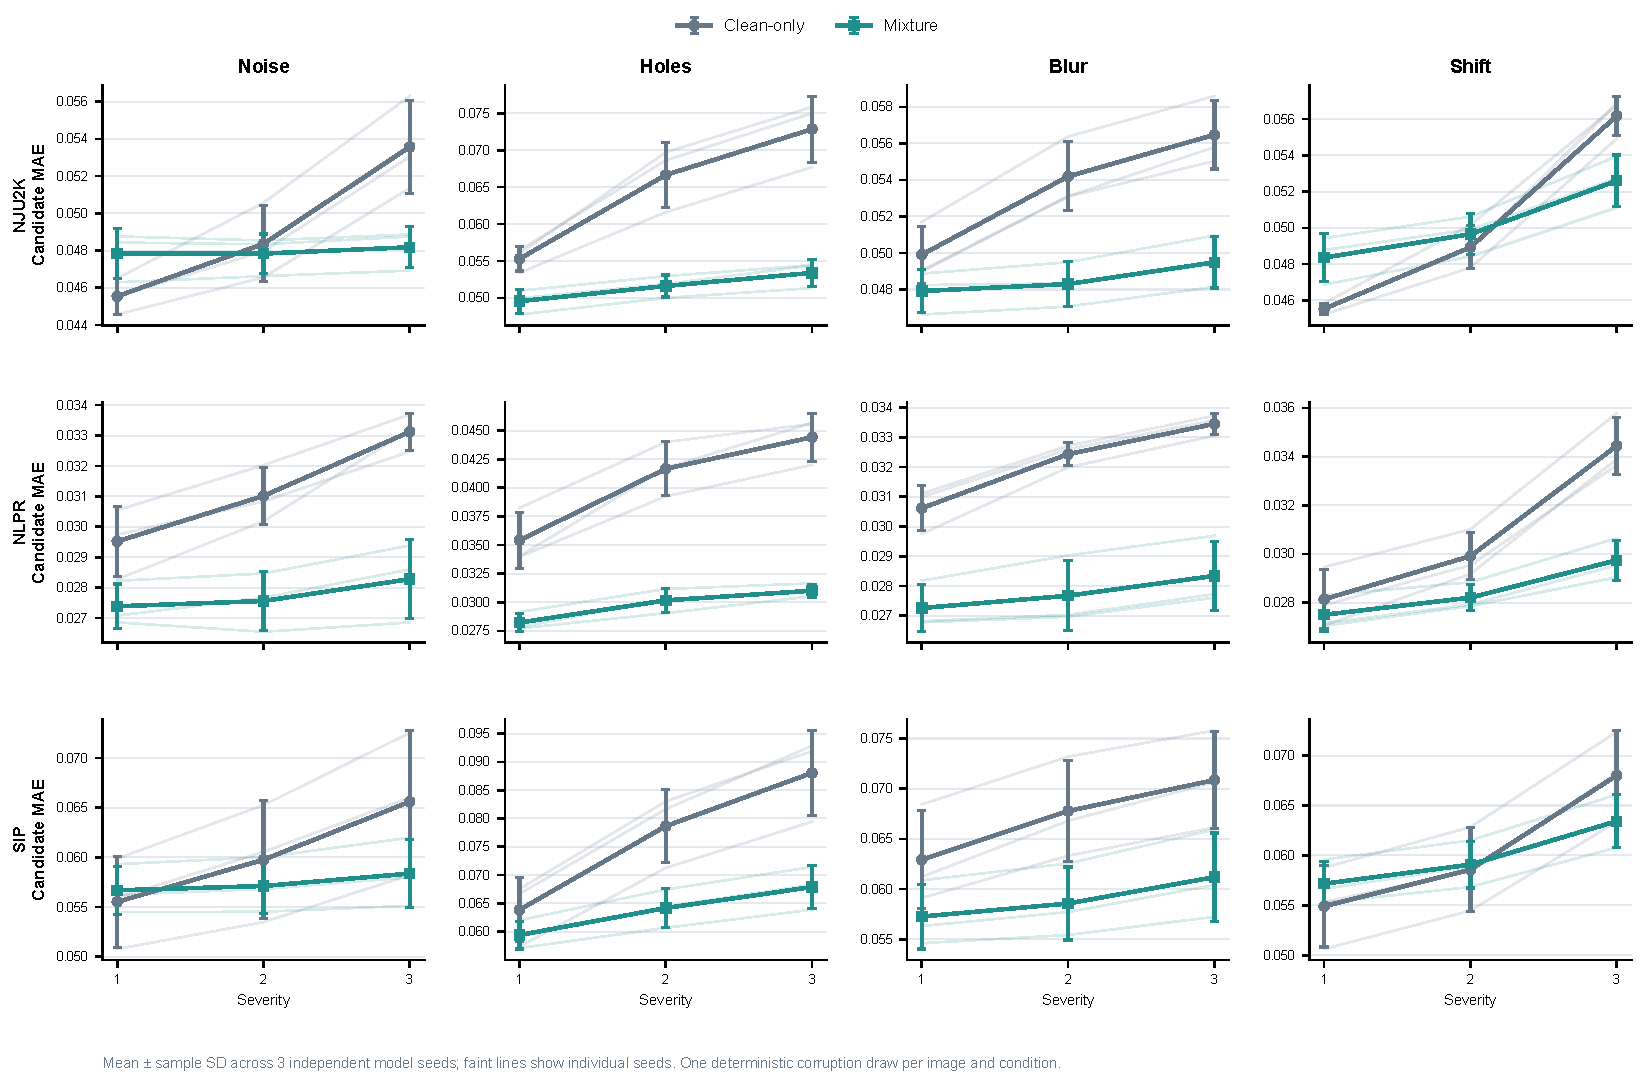
\includegraphics[width=\linewidth]{figure/fig3_corruption_training.pdf}
\caption{Candidate MAE under four depth-degradation families and three severities on NJU2K, NLPR, and SIP. Curves compare clean-only and corruption-mixture candidate training; bold points and error bars are the mean $\pm$ sample SD across three model seeds, and faint lines show individual seeds. Each image, condition, and seed has one deterministic perturbation realization. Complete removal is reported separately in Table~\ref{tab:families}.}
\label{fig:robustness}
\end{figure}

The degradation-family breakdown in Table~\ref{tab:families} shows the corruption-trained candidate remains better than the RGB reference on average for noise, holes, blur, and shift on all datasets. Under full depth removal, the ungated candidate is worse than RGB; the router reverts to the RGB output because validity is zero. Family values average the three severity levels and three seeds; removal has one level. These results concern simulated depth changes; sensor-level robustness remains untested.

Condition-wise results in Table~\ref{tab:conditions} reveal the expected severity trend: larger missing rectangles, stronger blur, and larger shifts generally increase candidate MAE. On NJU2K, for example, candidate MAE rises from 0.0495 to 0.0534 from holes severity 1 to 3; on SIP it rises from 0.0594 to 0.0679. The effect differs across perturbations. NJU2K noise changes candidate MAE little between severity 1 and 3 (0.0478 to 0.0482), whereas SIP shift raises it from 0.0572 to 0.0634. These comparisons locate the robustness boundary more clearly than an all-condition mean.

Complete depth removal is a distinct endpoint. The ungated candidate's mean MAE becomes 0.0592, 0.0337, and 0.0776 on NJU2K, NLPR, and SIP, worse than the respective RGB reference means. The availability rule sets every routing mask value to zero, recovering reference MAE 0.0557, 0.0316, and 0.0699. The fallback follows from the selector's validity rule. It does not show that the learned score detects partially unreliable depth.

\begin{table}[t]\centering\small
\caption{Mean MAE of the corruption-trained RGB-D candidate by test condition. The RGB-reference MAE is constant across depth perturbations within each dataset.}
\label{tab:families}
\begin{tabular}{lrrrrrr}\toprule Dataset & RGB & Noise & Holes & Blur & Shift & Removal\\\midrule
NJU2K & .0557 & .0479 & .0515 & .0486 & .0502 & .0592\\
NLPR & .0316 & .0277 & .0298 & .0278 & .0285 & .0337\\
SIP & .0699 & .0574 & .0638 & .0590 & .0599 & .0776\\\bottomrule\end{tabular}
\end{table}

\subsection{Router calibration and its limits}
The selected thresholds were $-0.10$, $-0.04$, and $0.02$ for seeds 17, 29, and 43. Their calibration selected-region fractions were 0.871, 0.858, and 0.057, respectively. The spread indicates that the learned score did not yield a stable selection rate across seeds. On clean test images, mean routed MAE was .0477, .0269, and .0570 for NJU2K, NLPR, and SIP. Under severe displacement, the mean positive test harm was $.0070\pm.0004$ on NJU2K and $.0061\pm.0003$ on SIP, both above the 0.005 calibration budget. NLPR was $.0042\pm.0012$. The router nevertheless returned exactly the RGB prediction when the depth-validity map was fully removed, and its reported benefit and harm were both zero for that condition.

\begin{table}[t]\centering\small
\caption{Routing controls under severe depth shift (severity 3), means $\pm$ SD over three seeds. Benefit is RGB MAE minus routed MAE; harm is mean positive per-image MAE excess relative to RGB.}
\label{tab:routing}
\begin{tabular}{llrrr}\toprule Dataset & Policy & Benefit & Positive harm & Selected fraction\\\midrule
NJU2K & Calibrated & $.0037\pm.0016$ & $.0070\pm.0004$ & $.6386\pm.4901$\\
 & Fixed $t=0$ & $.0034\pm.0018$ & $.0068\pm.0007$ & $.4884\pm.1205$\\
 & Validity-only & $.0030\pm.0022$ & $.0081\pm.0013$ & $.9267\pm.0013$\\\midrule
NLPR & Calibrated & $.0025\pm.0017$ & $.0042\pm.0012$ & $.6304\pm.5028$\\
 & Fixed $t=0$ & $.0026\pm.0012$ & $.0039\pm.0008$ & $.4907\pm.1156$\\
 & Validity-only & $.0019\pm.0013$ & $.0050\pm.0013$ & $.9254\pm.0023$\\\midrule
SIP & Calibrated & $.0068\pm.0007$ & $.0061\pm.0003$ & $.6387\pm.4809$\\
 & Fixed $t=0$ & $.0062\pm.0012$ & $.0058\pm.0012$ & $.4676\pm.1301$\\
 & Validity-only & $.0064\pm.0014$ & $.0074\pm.0009$ & $.9262\pm.0007$\\\bottomrule\end{tabular}
\end{table}

Figure~\ref{fig:routing} places the router's test benefit, positive harm, and depth-selection frequency side by side for clean depth, each severity-3 corruption, and complete removal. The dashed 0.005 line is the threshold-selection budget on calibration data, not a bound promised for the test sets.

\begin{figure}[!tbp]
\centering
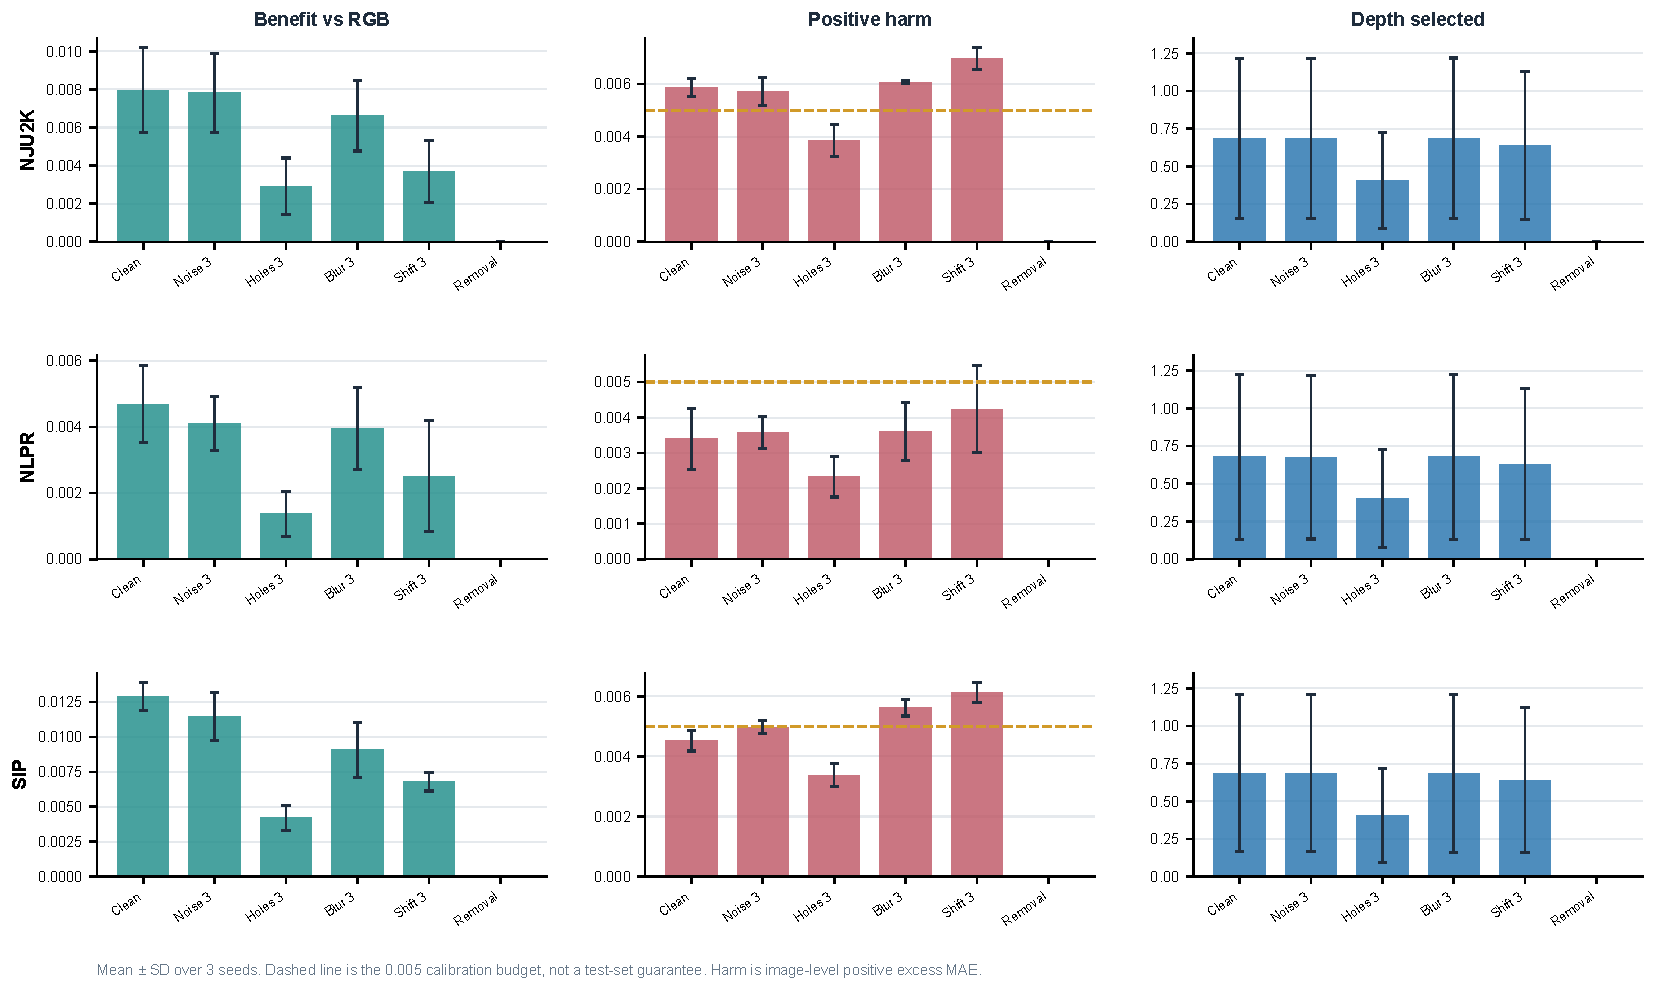
\includegraphics[width=\linewidth]{figure/fig4_router_diagnostics.pdf}
\caption{Held-out test diagnostics for the calibrated router. Each bar is the three-seed mean and each error bar the sample SD. Benefit is RGB MAE minus routed MAE; positive harm is the mean positive image-level excess MAE relative to RGB; depth selected is the fraction of regions using the RGB-D candidate. The dashed 0.005 line denotes an empirical calibration budget only. The plotted conditions are clean, severity 3 for each corruption family, and removal.}
\label{fig:routing}
\end{figure}

Fixed $t=0$ yielded similar benefit while often choosing fewer regions than the calibrated policy (Table~\ref{tab:routing}); the calibration experiment therefore does not show a decisive improvement over this simple control. Validity-only routing selected almost all available regions under shift and had greater positive harm. The router is therefore an evaluated selection mechanism, with no verified safety advantage.

The negative result is especially relevant because the calibration computation pools all fourteen conditions within each calibration image before applying the positive-part operator. Harm under one condition can be offset by benefit under another for the same image. Test reporting instead computes positive excess separately for each condition, exposing the severe-shift cases. The budget also depends on the fixed calibration pool and the model seed. A reliable operating guarantee would require a differently specified target risk, assumptions on future data, and a validated control rule. Table~\ref{tab:calibration} reports the observed calibration behavior; no formal risk-control claim follows from it. Figure~\ref{fig:qualitative} shows actual test-image predictions, including harmful depth and a router failure. In this seed the route mask often selects the entire candidate map, whereas full removal forces the RGB fallback; the examples therefore reinforce the measured seed sensitivity rather than suggesting a reliably selective gate.

\begin{figure}[!tbp]
\centering
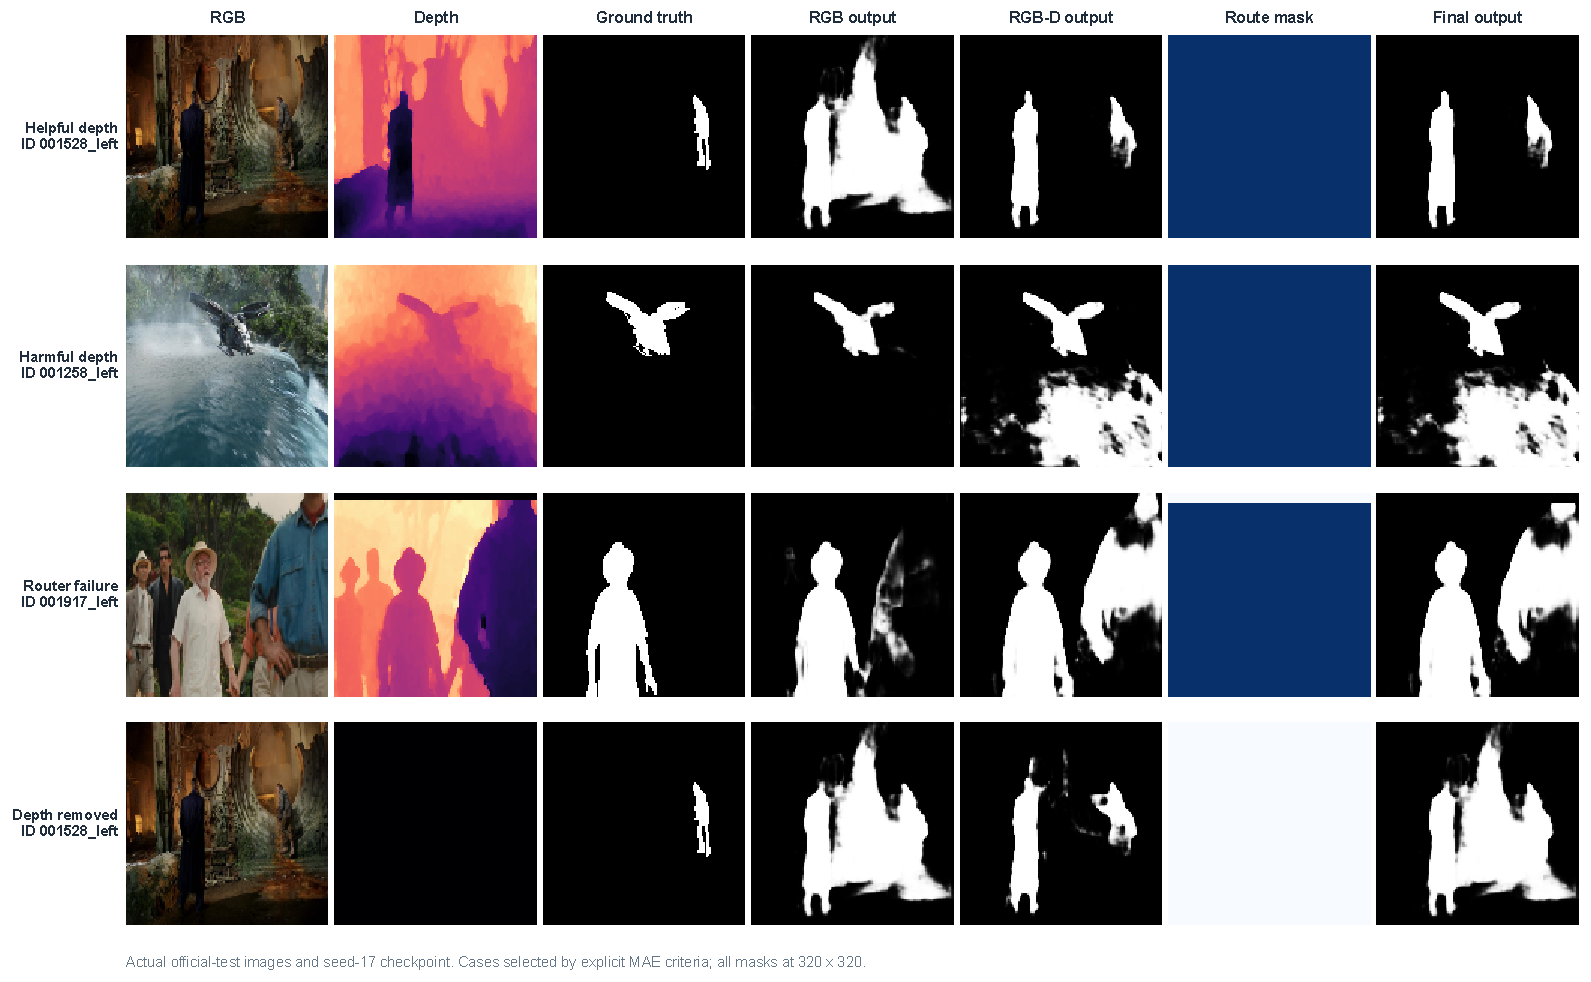
\includegraphics[width=\linewidth]{figure/fig5_qualitative.pdf}
\caption{Qualitative predictions from the official NJU2K test set using the seed-17 checkpoint. Rows are selected by explicit per-image MAE criteria: helpful clean depth, harmful clean depth, severe-shift router failure, and complete depth removal. Columns show RGB, depth, ground truth, RGB output, RGB-D output, the selected-region mask (blue denotes RGB-D selection), and routed output. Sample IDs appear in the figure; the first and last rows intentionally reuse one image to demonstrate the missing-depth fallback.}
\label{fig:qualitative}
\end{figure}

\subsection{Inference cost}
The full system evaluates both predictors before routing. On the local RTX 3060 Laptop GPU at batch size one and $320\times320$ inputs, 100 synchronized timed iterations after 10 warmups gave the values in Table~\ref{tab:efficiency}. The full system was about three times slower than the RGB reference. These are forward-pass measurements; file I/O, image decoding, and corruption generation were excluded.

The router adds comparatively few parameters, but it cannot decide between predictors without evaluating both. Therefore, the full system carries approximately 33.8 million parameters, compared with 22.5 million for the candidate alone, and its measured 28.57 ms mean latency is higher than the sum of simple single-model deployment expectations. These measurements quantify the accuracy--compute trade-off. Whether the resulting throughput is usable depends on the application.

\begin{table}[t]\centering\small
\caption{Mean over three seed checkpoints for synchronized batch-1 inference. Peak allocated GPU memory is measured within the timing process.}
\label{tab:efficiency}
\begin{tabular}{lrrrr}\toprule Model & Parameters & Mean ms & p95 ms & Images/s\\\midrule
RGB reference & 11,262,881 & 9.32 & 14.51 & 107.5\\
RGB-D candidate & 22,546,465 & 17.56 & 26.10 & 57.3\\
Both predictors + router & 33,821,283 & 28.57 & 40.77 & 35.6\\\bottomrule\end{tabular}
\end{table}


\section{Discussion}
The clearest finding comes from the repeated candidate-training comparison: across all three seeds and three test datasets, the average of the specified degraded conditions favors corruption-mixture training. The result documents a repeatable benefit of the specified training policy on these benchmarks. The comparison is especially informative because fitting split, architecture, optimizer, epoch count, test images, and deterministic perturbations were held fixed. Its causal interpretation is still limited by independently sampled decoder/fusion initializations and by the fact that the synthetic corruptions were fixed per training image rather than resampled every epoch.

\subsection{Contribution boundary}
The defensible innovation is the measured combination of a deliberately specified training perturbation policy and an auditable candidate-relative selection experiment. Corruption augmentation, RGB-D fusion, and reliability gating have substantial prior art; none is presented as a new primitive. Our data isolate the candidate-training result more convincingly than the router result because the clean-only ablation directly compares the same architecture under two input policies, whereas the calibrated router does not consistently improve upon a simple fixed threshold. The router is best understood here as a diagnostic experiment: the fixed threshold performs similarly, and its result is part of the comparison.

The observed corruption-training gain is also architecture-specific. The candidate contains a dual ResNet-18 pathway, a simple multi-scale fusion block, and a conventional decoder. It is plausible that a stronger quality-aware model could show a different magnitude or even a different sign of benefit from this exact mixture. Since no such model was retrained here, the paper can recommend the protocol as a reproducible evaluation pattern but cannot generalize its measured gain to all RGB-D detectors.

The router results are less consistent. Complete missing-depth fallback works by construction and was observed in the test summaries. However, calibrated selection was seed-sensitive, offered little consistent improvement over a fixed threshold, and exceeded its calibration harm budget on severe-shift NJU2K and SIP tests. The low calibration harm reflects that split and its averaging rule, not a safety certificate. The difference between averaging before clipping in calibration and clipping each test condition separately further cautions against direct numerical equivalence.

\subsection{Why test harm can exceed the budget}
The budget is a threshold-selection criterion, not an estimate of the worst-case effect of routing. A positive-harm mean can increase when the distribution of signed image differences changes, even when average routed MAE remains below RGB MAE. Under severe shift, depth content is displaced relative to RGB and ground truth, a failure mode for which the candidate and router need not react in the same way. The validity fraction remains high except at newly exposed borders; a validity-only selector therefore cannot detect the interior misregistration. The learned utility router uses disagreement and depth gradients, but the results show these features are insufficient for a stable harm ceiling. This interpretation is consistent with the high selected fractions and the severe-shift harm values in Table~\ref{tab:routing}; it is an inference about the implemented features, not a proven causal diagnosis.

Several limitations shape the scope of these findings. The reported masks and metrics use resized 320$\times$320 inputs, not native-resolution benchmark outputs. Noise, holes, blur, and shift probe sensitivity in an 8-bit normalized depth representation; they are not validated camera-noise models. The reference and candidate are both executed for routing, increasing parameters and latency. Hard $16\times16$ region decisions may produce block boundaries, which have not yet been quantified visually. Finally, no retrained external SOD model was included under the matched protocol, so the paper cannot claim state-of-the-art performance. Future work should first compare externally implemented models under identical training and perturbations, then revisit routing with a less seed-sensitive score and an explicitly specified risk-control procedure.

\section{Conclusion}
On three RGB-D saliency test sets and three training seeds, the implemented depth-corruption mixture improved candidate MAE under the thirteen specified degraded conditions relative to clean-only training. The independent RGB reference supplied a reliable functional fallback when depth was wholly absent. A candidate-relative utility router was implemented and measured, but its threshold behavior and severe-shift harm did not support a general 0.005 safety claim or a clear advantage over fixed-threshold routing. The main supported result is the robustness gain from the specified training policy. Reliable routing remains unresolved.

\section*{Data and Code Availability}
Code, exact train/validation/calibration and test manifests with source-file hashes, per-image evaluation metrics, calibration records, aggregate results, and figure sources are available in the public repository \url{https://github.com/wunan-snsy/A-Three-Seed-Study-with-an-Audited-Regional-Router}. The tagged release \texttt{v1.0.0} identifies the archived version used for this manuscript. Original NJU2K, NLPR, and SIP images are not redistributed; readers must obtain them from the benchmark providers under the applicable terms and place them at the relative paths recorded in the manifests. Full-precision model checkpoints are not included in this release and can be regenerated using the provided training scripts and recorded seeds. The numerical results can be traced to \path{results/formal_seed17/test_seed17_full/evaluation.csv}, \path{results/formal_seed17/test_seed17_full/per_image_metrics.csv}, and \path{results/ablation_clean_candidate_seed17/paired_candidate_summary.csv}, with corresponding files for seeds 29 and 43. Two large per-image CSV files are stored losslessly as \texttt{.csv.gz}, as noted in the repository README. The preprocessing, corruption, training, evaluation, and plotting scripts are under \texttt{src/} and \texttt{figures/}; the executed settings are recorded in \path{config/executed_protocol.json}.

\section*{Declarations}
Author contributions, funding, and competing-interest declarations: [TO BE SUPPLIED BY AUTHORS].


\appendix
\section{Full condition-wise MAE record}
Table~\ref{tab:conditions} gives the mean over three seeds for every evaluated condition. It preserves the high-shift and removal outcomes that would be obscured by a single corruption average. These are resized-mask MAE values, with one deterministic perturbation realization per image, condition, and seed. The CSV files named in the availability statement contain the corresponding per-seed and per-image records.

\small
\begin{longtable}{llrrrrr}
\caption{Condition-wise three-seed mean MAE and positive routed harm at 320$\times$320. Severity 0 denotes clean depth or complete removal; severities 1--3 follow the perturbation definitions.}\label{tab:conditions}\\
\toprule Dataset & Condition & Sev. & RGB & RGB-D & Routed & Harm\\\midrule
\endfirsthead
\toprule Dataset & Condition & Sev. & RGB & RGB-D & Routed & Harm\\\midrule
\endhead
\bottomrule
\endfoot
NJU2K & Clean & 0 & 0.0557 & 0.0479 & 0.0477 & 0.0059\\
NJU2K & Noise & 1 & 0.0557 & 0.0478 & 0.0476 & 0.0058\\
NJU2K & Noise & 2 & 0.0557 & 0.0478 & 0.0476 & 0.0058\\
NJU2K & Noise & 3 & 0.0557 & 0.0482 & 0.0478 & 0.0057\\
NJU2K & Holes & 1 & 0.0557 & 0.0495 & 0.0492 & 0.0056\\
NJU2K & Holes & 2 & 0.0557 & 0.0516 & 0.0510 & 0.0046\\
NJU2K & Holes & 3 & 0.0557 & 0.0534 & 0.0527 & 0.0038\\
NJU2K & Blur & 1 & 0.0557 & 0.0479 & 0.0476 & 0.0057\\
NJU2K & Blur & 2 & 0.0557 & 0.0483 & 0.0479 & 0.0058\\
NJU2K & Blur & 3 & 0.0557 & 0.0495 & 0.0490 & 0.0061\\
NJU2K & Shift & 1 & 0.0557 & 0.0484 & 0.0480 & 0.0059\\
NJU2K & Shift & 2 & 0.0557 & 0.0497 & 0.0491 & 0.0061\\
NJU2K & Shift & 3 & 0.0557 & 0.0526 & 0.0520 & 0.0070\\
NJU2K & Removal & 0 & 0.0557 & 0.0592 & 0.0557 & 0.0000\\
NLPR & Clean & 0 & 0.0316 & 0.0273 & 0.0269 & 0.0034\\
NLPR & Noise & 1 & 0.0316 & 0.0274 & 0.0269 & 0.0035\\
NLPR & Noise & 2 & 0.0316 & 0.0276 & 0.0270 & 0.0034\\
NLPR & Noise & 3 & 0.0316 & 0.0283 & 0.0275 & 0.0036\\
NLPR & Holes & 1 & 0.0316 & 0.0282 & 0.0278 & 0.0031\\
NLPR & Holes & 2 & 0.0316 & 0.0302 & 0.0297 & 0.0030\\
NLPR & Holes & 3 & 0.0316 & 0.0310 & 0.0302 & 0.0023\\
NLPR & Blur & 1 & 0.0316 & 0.0273 & 0.0268 & 0.0034\\
NLPR & Blur & 2 & 0.0316 & 0.0277 & 0.0270 & 0.0035\\
NLPR & Blur & 3 & 0.0316 & 0.0283 & 0.0276 & 0.0036\\
NLPR & Shift & 1 & 0.0316 & 0.0275 & 0.0270 & 0.0035\\
NLPR & Shift & 2 & 0.0316 & 0.0282 & 0.0277 & 0.0037\\
NLPR & Shift & 3 & 0.0316 & 0.0297 & 0.0291 & 0.0042\\
NLPR & Removal & 0 & 0.0316 & 0.0337 & 0.0316 & 0.0000\\
SIP & Clean & 0 & 0.0699 & 0.0567 & 0.0570 & 0.0045\\
SIP & Noise & 1 & 0.0699 & 0.0567 & 0.0571 & 0.0046\\
SIP & Noise & 2 & 0.0699 & 0.0571 & 0.0575 & 0.0047\\
SIP & Noise & 3 & 0.0699 & 0.0584 & 0.0585 & 0.0050\\
SIP & Holes & 1 & 0.0699 & 0.0594 & 0.0597 & 0.0043\\
SIP & Holes & 2 & 0.0699 & 0.0642 & 0.0630 & 0.0040\\
SIP & Holes & 3 & 0.0699 & 0.0679 & 0.0657 & 0.0034\\
SIP & Blur & 1 & 0.0699 & 0.0573 & 0.0575 & 0.0047\\
SIP & Blur & 2 & 0.0699 & 0.0586 & 0.0586 & 0.0049\\
SIP & Blur & 3 & 0.0699 & 0.0612 & 0.0609 & 0.0056\\
SIP & Shift & 1 & 0.0699 & 0.0572 & 0.0575 & 0.0046\\
SIP & Shift & 2 & 0.0699 & 0.0591 & 0.0591 & 0.0050\\
SIP & Shift & 3 & 0.0699 & 0.0634 & 0.0631 & 0.0061\\
SIP & Removal & 0 & 0.0699 & 0.0776 & 0.0699 & 0.0000\\
\end{longtable}
\normalsize

\section{Seed-wise training-policy contrast}
Table~\ref{tab:seedablation} retains each independent fit rather than treating three model seeds as if they were independent test images. The difference uses the mean of 13 degraded conditions for each image before averaging over images. Confidence intervals resample image IDs within a seed, preserving the matched corruption conditions; their width therefore addresses image sampling, whereas the seed-to-seed variation appears as three separate rows per dataset.

\begin{table}[htbp]\centering\small
\caption{Candidate-training ablation by model seed. $\Delta=$ clean-only MAE minus corruption-trained MAE, averaged over all 13 degraded conditions. CI is the paired image-bootstrap 95\% interval (5,000 resamples).}
\label{tab:seedablation}
\begin{tabular}{lrrrrr}\toprule Dataset & Seed & Corrupt. train & Clean-only & $\Delta$ & 95\% CI for $\Delta$\\\midrule
NJU2K & 17 & 0.0487 & 0.0536 & 0.0048 & [0.0020, 0.0077]\\
NJU2K & 29 & 0.0515 & 0.0557 & 0.0042 & [0.0010, 0.0071]\\
NJU2K & 43 & 0.0506 & 0.0571 & 0.0065 & [0.0037, 0.0092]\\
NLPR & 17 & 0.0282 & 0.0335 & 0.0052 & [0.0025, 0.0083]\\
NLPR & 29 & 0.0298 & 0.0352 & 0.0053 & [0.0022, 0.0081]\\
NLPR & 43 & 0.0285 & 0.0336 & 0.0051 & [0.0023, 0.0080]\\
SIP & 17 & 0.0582 & 0.0622 & 0.0039 & [0.0021, 0.0056]\\
SIP & 29 & 0.0647 & 0.0688 & 0.0040 & [0.0016, 0.0063]\\
SIP & 43 & 0.0612 & 0.0729 & 0.0117 & [0.0096, 0.0138]\\
\bottomrule\end{tabular}
\end{table}

\section{Calibration details and interpretation}
For transparency, Table~\ref{tab:calibration} lists the actual seed-specific thresholds and within-calibration quantities. The calibration score pools fourteen conditions within each of 218 images before computing positive harm; each test row in Table~\ref{tab:conditions} instead describes a single condition. The threshold was not changed after viewing the official test sets.

\begin{table}[htbp]\centering\small
\caption{Held-out calibration output by seed. Benefit and positive harm are absolute MAE differences from the RGB reference. Selection is the mean fraction of regions routed to RGB-D in calibration.}
\label{tab:calibration}
\begin{tabular}{rrrrr}\toprule Seed & Threshold & Benefit & Positive harm & Selected fraction\\\midrule
17 & -0.10 & 0.0068 & 0.0044 & 0.871\\
29 & -0.04 & 0.0033 & 0.0050 & 0.858\\
43 & 0.02 & 0.0053 & 0.0039 & 0.057\\
\bottomrule\end{tabular}
\end{table}

\small
% Bibliography entries below are selected from the author's source manuscript and retain DOI/source identifiers.
% Full bibliographic metadata should be checked against the publisher record before submission.
\begin{thebibliography}{99}
\bibitem{d3net} D. Fan, Z. Lin, J. Zhao, Y. Liu, Z. Zhang, Q. Hou, M. Zhu, M. Cheng, ``Rethinking RGB-D Salient Object Detection: Models, Data Sets, and Large-Scale Benchmarks," IEEE Transactions on Neural Networks and Learning Systems, 2021. DOI:10.1109/TNNLS.2020.2996406.
\bibitem{survey2021} T. Zhou, D. Fan, M. Cheng, J. Shen, L. Shao, ``RGB-D salient object detection: A survey," Computational Visual Media, 2021. DOI:10.1007/s41095-020-0199-z.
\bibitem{pcf} H. Chen, Y. Li, ``Progressively Complementarity-Aware Fusion Network for RGB-D Salient Object Detection," 2018 IEEE/CVF Conference on Computer Vision and Pattern Recognition, 2018. DOI:10.1109/CVPR.2018.00322.
\bibitem{dmra} Y. Piao, W. Ji, J. Li, M. Zhang, H. Lu, ``Depth-Induced Multi-Scale Recurrent Attention Network for Saliency Detection," IEEE International Conference on Computer Vision, 2019. DOI:10.1109/ICCV.2019.00735.
\bibitem{jldcf} K. Fu, D. Fan, G. Ji, Q. Zhao, ``JL-DCF: Joint Learning and Densely-Cooperative Fusion Framework for RGB-D Salient Object Detection," Computer Vision and Pattern Recognition, 2020. DOI:10.1109/cvpr42600.2020.00312.
\bibitem{bbsnet} D. Fan, Y. Zhai, A. Borji, J. Yang, L. Shao, ``BBS-Net: RGB-D Salient Object Detection with a Bifurcated Backbone Strategy Network," European Conference on Computer Vision, 2020. DOI:10.1007/978-3-030-58610-2\_17.
\bibitem{dcf} W. Ji, J. Li, S. Yu, M. Zhang, Y. Piao, S. Yao, Q. Bi, K. Ma, Y. Zheng, H. Lu, L. Cheng, ``Calibrated RGB-D Salient Object Detection," Computer Vision and Pattern Recognition, 2021. DOI:10.1109/CVPR46437.2021.00935.
\bibitem{dqas} C. Chen, J. Wei, C. Peng, H. Qin, ``Depth-Quality-Aware Salient Object Detection," IEEE Transactions on Image Processing, 2021. DOI:10.1109/TIP.2021.3052069.
\bibitem{dqfm} W. Zhang, G. Ji, Z. Wang, K. Fu, Q. Zhao, ``Depth Quality-Inspired Feature Manipulation for Efficient RGB-D Salient Object Detection," ACM Multimedia, 2021. DOI:10.1145/3474085.3475240.
\bibitem{dsn} H. Wen, C. Yan, X. Zhou, R. Cong, Y. Sun, B. Zheng, J. Zhang, Y. Bao, G. Ding, ``Dynamic Selective Network for RGB-D Salient Object Detection," IEEE Transactions on Image Processing, 2021. DOI:10.1109/TIP.2021.3123548.
\bibitem{twophase} C. Chen, J. Wei, C. Peng, W. Zhang, H. Qin, ``Improved Saliency Detection in RGB-D Images Using Two-Phase Depth Estimation and Selective Deep Fusion," IEEE Transactions on Image Processing, 2020. DOI:10.1109/TIP.2020.2968250.
\bibitem{cmms} C. Li, R. Cong, Y. Piao, Q. Xu, C. C. Loy, ``RGB-D Salient Object Detection with Cross-Modality Modulation and Selection," European Conference on Computer Vision, 2020. DOI:10.1007/978-3-030-58598-3\_14.
\bibitem{a2dele} Y. Piao, Z. Rong, M. Zhang, W. Ren, H. Lu, ``A2dele: Adaptive and Attentive Depth Distiller for Efficient RGB-D Salient Object Detection," Computer Vision and Pattern Recognition, 2020. DOI:10.1109/CVPR42600.2020.00908.
\bibitem{mobilesal} Y. Wu, Y. Liu, J. Xu, J. Bian, Y. Gu, M. Cheng, ``MobileSal: Extremely Efficient RGB-D Salient Object Detection," IEEE Transactions on Pattern Analysis and Machine Intelligence, 2022. DOI:10.1109/TPAMI.2021.3134684.
\bibitem{selectivenet} Y. Geifman and R. El-Yaniv, ``SelectiveNet: A Deep Neural Network with an Integrated Reject Option," ICML, 2019.
\bibitem{guo2017} C. Guo, G. Pleiss, Y. Sun, and K. Q. Weinberger, ``On Calibration of Modern Neural Networks," ICML, 2017.
\bibitem{smeasure} D.-P. Fan, M.-M. Cheng, Y. Liu, T. Li, and A. Borji, ``Structure-measure: A New Way to Evaluate Foreground Maps," ICCV, 2017. DOI:10.1109/ICCV.2017.454.
\bibitem{weighted} R. Margolin, L. Zelnik-Manor, and A. Tal, ``How to Evaluate Foreground Maps?," CVPR, 2014. DOI:10.1109/CVPR.2014.39.
\bibitem{emeasure} D.-P. Fan, C. Gong, Y. Cao, B. Ren, M.-M. Cheng, and A. Borji, ``Enhanced-alignment Measure for Binary Foreground Map Evaluation," IJCAI, 2018. DOI:10.24963/ijcai.2018/97.
\bibitem{resnet} K. He, X. Zhang, S. Ren, and J. Sun, ``Deep Residual Learning for Image Recognition," CVPR, 2016. DOI:10.1109/CVPR.2016.90.
\bibitem{vst} N. Liu, N. Zhang, K. Wan, L. Shao, J. Han, ``Visual Saliency Transformer," IEEE International Conference on Computer Vision, 2021. DOI:10.1109/ICCV48922.2021.00468.
\bibitem{crossview} J. Han, H. Chen, N. Liu, C. Yan, X. Li, ``CNNs-Based RGB-D Saliency Detection via Cross-View Transfer and Multiview Fusion," IEEE Transactions on Cybernetics, 2018. DOI:10.1109/TCYB.2017.2761775.
\bibitem{swinnet} Z. Liu, Y. Tan, Q. He, Y. Xiao, ``SwinNet: Swin Transformer Drives Edge-Aware RGB-D and RGB-T Salient Object Detection," IEEE transactions on circuits and systems for video technology (Print), 2022. DOI:10.1109/TCSVT.2021.3127149.
\bibitem{mmci} H. Chen, Y. Li, D. Su, ``Multi-modal fusion network with multi-scale multi-path and cross-modal interactions for RGB-D salient object detection," Pattern Recognition, 2019. DOI:10.1016/j.patcog.2018.08.007.
\bibitem{tanse} H. Chen, Y. Li, ``Three-Stream Attention-Aware Network for RGB-D Salient Object Detection," IEEE Transactions on Image Processing, 2019. DOI:10.1109/TIP.2019.2891104.
\bibitem{hainet} G. Li, Z. Liu, M. Chen, Z. Bai, W. Lin, H. Ling, ``Hierarchical Alternate Interaction Network for RGB-D Salient Object Detection," IEEE Transactions on Image Processing, 2021. DOI:10.1109/TIP.2021.3062689.
\bibitem{singlestream} X. Zhao, L. Zhang, Y. Pang, H. Lu, L. Zhang, ``A Single Stream Network for Robust and Real-time RGB-D Salient Object Detection," European Conference on Computer Vision, 2020. DOI:10.1007/978-3-030-58542-6\_39.
\bibitem{siamese} K. Fu, D. Fan, G. Ji, Q. Zhao, J. Shen, C. Zhu, ``Siamese Network for RGB-D Salient Object Detection and Beyond," IEEE Transactions on Pattern Analysis and Machine Intelligence. DOI:10.1109/TPAMI.2021.3073689.
\bibitem{icnet} G. Li, Z. Liu, H. Ling, ``ICNet: Information Conversion Network for RGB-D Based Salient Object Detection," IEEE Transactions on Image Processing, 2020. DOI:10.1109/TIP.2020.2976689.
\bibitem{hdfnet} Y. Pang, L. Zhang, X. Zhao, H. Lu, ``Hierarchical Dynamic Filtering Network for RGB-D Salient Object Detection," European Conference on Computer Vision, 2020. DOI:10.1007/978-3-030-58595-2\_15.
\bibitem{ssf} M. Zhang, W. Ren, Y. Piao, Z. Rong, H. Lu, ``Select, Supplement and Focus for RGB-D Saliency Detection," Computer Vision and Pattern Recognition, 2020. DOI:10.1109/CVPR42600.2020.00353.
\bibitem{lbe} D. Feng, N. Barnes, S. You, C. McCarthy, ``Local Background Enclosure for RGB-D Salient Object Detection," Computer Vision and Pattern Recognition, 2016. DOI:10.1109/CVPR.2016.257.
\bibitem{dpanet} Z. Chen, R. Cong, Q. Xu, Q. Huang, ``DPANet: Depth Potentiality-Aware Gated Attention Network for RGB-D Salient Object Detection," IEEE Transactions on Image Processing, 2020. DOI:10.1109/TIP.2020.3028289.
\bibitem{cirnet} R. Cong, Q. Lin, C. Zhang, C. Li, X. Cao, Q. Huang, Y. Zhao, ``CIR-Net: Cross-Modality Interaction and Refinement for RGB-D Salient Object Detection," IEEE Transactions on Image Processing, 2022. DOI:10.1109/TIP.2022.3216198.
\bibitem{caver} Y. Pang, X. Zhao, L. Zhang, H. Lu, ``CAVER: Cross-Modal View-Mixed Transformer for Bi-Modal Salient Object Detection," IEEE Transactions on Image Processing, 2023. DOI:10.1109/TIP.2023.3234702.
\bibitem{globalprior} J. Ren, X. Gong, L. Yu, W. Zhou, M. Yang, ``Exploiting global priors for RGB-D saliency detection," 2015 IEEE Conference on Computer Vision and Pattern Recognition Workshops (CVPRW), 2015. DOI:10.1109/CVPRW.2015.7301391.
\bibitem{conet} W. Ji, J. Li, M. Zhang, Y. Piao, H. Lu, ``Accurate RGB-D Salient Object Detection via Collaborative Learning," European Conference on Computer Vision, 2020. DOI:10.1007/978-3-030-58523-5\_4.
\bibitem{tritrans} Z. Liu, Y. Wang, Z. Tu, Y. Xiao, B. Tang, ``TriTransNet: RGB-D Salient Object Detection with a Triplet Transformer Embedding Network," ACM Multimedia, 2021. DOI:10.1145/3474085.3475601.
\bibitem{rd3d} Q. Chen, Z. Liu, Y. Zhang, K. Fu, Q. Zhao, H. Du, ``RGB-D Salient Object Detection via 3D Convolutional Neural Networks," AAAI Conference on Artificial Intelligence, 2021. DOI:10.1609/aaai.v35i2.16191.
\bibitem{cdnet} W. Jin, J. Xu, Q. Han, Y. Zhang, M. Cheng, ``CDNet: Complementary Depth Network for RGB-D Salient Object Detection," IEEE Transactions on Image Processing, 2021. DOI:10.1109/TIP.2021.3060167.
\bibitem{moadnet} X. Jin, K. Yi, J. Xu, ``MoADNet: Mobile Asymmetric Dual-Stream Networks for Real-Time and Lightweight RGB-D Salient Object Detection," IEEE transactions on circuits and systems for video technology (Print), 2022. DOI:10.1109/TCSVT.2022.3180274.
\bibitem{calibrateddepth} J. Li, W. Ji, M. Zhang, Y. Piao, H. Lu, L. Cheng, ``Delving into Calibrated Depth for Accurate RGB-D Salient Object Detection," International Journal of Computer Vision. DOI:10.1007/s11263-022-01734-1.
\end{thebibliography}
\end{document}
